% Définir les expressions régulières, definir la "finalité" de e f(e), comme 1 si e contient le mot vide et 0 sinon.
% Définir le graphe (pointé) d'antimirov d'une regexp. Il ne faut pas l'appeller automate plutôt que graphe
% Définir la bisimulation entre deux graphes (pointés), donner des exemples
% Rapelle l'axiomatisation de Salooma. Le système de Salooma axiomatise l'egalité des langages d'expressions régulières. Rapelle tout ce qu'il faut pour définir l'axiomatisabilité et tout ça. Je ne sais pas s'il faut faire des defs generiques sur l'axiomatisatbilité d'une relation sur les regexp en général ou être plus specifique à ce cas?
% Définir un système de Salooma modifié, que tu appelleras le système de Milner. La différence avec Salooma c'est qu'il y a la règle de distributivité à gauche (e+f)g=ef+eg mais pas la distributivité à droite (cad e(f+g)=ef+eg). Et garde seulement la loi e*=ee*+1 et enlève la loi e*=e*e+1.  Je l'appelle Système Milner car ce dernier a posé la question de s'il suffisait à axiomatiser la bisimulation. Note la prouvabilité e==f (remplace le == par un signe \equiv)
% Enoncer le théorème qu'on va montrer: Le système de Milner axiomatise la bisimulation entre regexp.

% Les ingrédients:

% Le premier ingrédient:
% On décrit un système de réecriture sur les graphes. 
% Là tu dois me mettre trois règles: la première correspond à la state élimination sauf que ici, l'état à éliminer a une unique arrête sortante qui n'est pas une self loop. La deuxième opération transforme deux arêtes parallèle en une unique arête, La troisième prend un état p qui a potentiellement plusieurs fils, ajoute un nouvel état q qui a comme ensemble de fils un sous ensemble S des fils de q , ajoute une transition de p vers q, et enlève les éléments de S de l'ensemble des fils de p.

% Ensuite  on normalise un graphe en  rajoutant un état initial et un état final comme on fait d'habitude. On dit qu'un graphe est réductible si sa normalisation se résuit vers: (mettre le graphe  
% Proposition 1: Si G est le graphe d'une regexp alors G est  réductible 
% (La réciproque est vrai aussi :Si un graphe est réductible alors c'est le graphe d'une expression mais on en a pas besoin pour la preuve du théorème principal, on le démontrera à la fin).

% La deuxième notion importante:
% Une décoration compatible d'un graphe c'est un étiquetage d'un graphe avec regexp, de telle sorte que pour toute etiquette e dont les fils sont e_1, ...e_n, on a (e==e_1+...+e_n +f(e)).
% Proposition: Si un graph a deux décorations compatibles, alors e==f où e et f sont les racines de la décoration. 

% Le troisième ingrédient:
% Je dit qu'un graphe est compacte s'il n'a pas deux états distincts et bisimilaires. En partant d'un graphe quelquonque, on obtient un compact en fusionnant ses états bisimilaires. On appelle ça la compactification.

% Le troisième résultat est que la compactification d'une regexp est une regexp. 

% Voici comment on rassembler ces ingrédients: Tout d'abord on montre que pour toutes les reg exp compactes, si elles sont bisimilaires, elles sont prouvables, en effet, si elle sont bisimilaires elles ont le même graphe, ce qui donne deux décorations compatibles pour ce graphe, et donc les expressions sont prouvablement équivalentes.

% Maintenant si e est une expression quelquonque et c une regexp pour sa compactification, il est facile de voir que c et ses dérivées forment une décoration compatible pour le graphe de e. Evidememnt e lui même induit une décoration compatible de son graphe. Comme G est le graphe de e il est réductible (prop1) et donc e==c. CE qui achève la preuve.  

\documentclass{article}
\usepackage[utf8]{inputenc}
\usepackage{amsmath}
\usepackage{amssymb}
\usepackage{amsthm}
\usepackage{stmaryrd}
\usepackage{graphicx}
\usepackage{csquotes}
\usepackage{tikz}
\usetikzlibrary{automata, positioning}
\usepackage{hyperref}
\usepackage{mathtools}
\hypersetup{
    colorlinks=true,
    linkcolor=blue,
    filecolor=magenta,      
    urlcolor=blue,
    citecolor=blue,
    pdfborder={0 0 0} % Removes the red boxes around links
}
\usepackage{listings}
\usepackage{tikz}
\usetikzlibrary{automata, positioning, arrows.meta, shapes, arrows}
% For better listings
\usepackage{listings}
% For mathbb, mathcal, etc.
\usepackage{amsfonts}
% For clever referencing (optional, but useful)
\usepackage{cleveref}
\usepackage{lmodern,amsmath,amssymb}
%for lowercase calligraphic math
\usepackage{boondox-cal}%for lowercase \mathcal
\usetikzlibrary{arrows.meta,positioning,calc}
\usetikzlibrary{decorations.pathmorphing}
\tikzset{
  state/.style={draw,rectangle,minimum size=2.5mm,inner sep=0pt},
  circ/.style={draw,circle,minimum size=1.5mm,inner sep=0pt, fill=black},
trig/.style={draw,regular polygon,regular polygon sides=3,shape border rotate=180,minimum size=2.5mm,inner sep=0pt},
  hub/.style={state,dashed},
  arr/.style={-{Latex[length=1.6mm]},line width=0.4pt},
  lab/.style={font=\scriptsize,inner sep=1pt,fill=white,fill opacity=.9,text opacity=1},
  ruletitle/.style={font=\bfseries\scriptsize}
}




\newtheorem{definition}{Definition}[section]
\newtheorem{lemma}[definition]{Lemma}
\newtheorem{proposition}[definition]{Proposition}
\newtheorem{theorem}[definition]{Theorem}
\newtheorem{claim}[definition]{Claim}
\newtheorem{corollary}[definition]{Corollary}
\newtheorem{remark}[definition]{Remark}
\newtheorem{example}[definition]{Example}

\newcommand{\A}{\mathcal{A}}
\newcommand{\B}{\mathcal{B}}

\begin{document}
\title{Axiomatization of Bisimulation for Regular Expressions}
\author{Your Name}
\date{\today}
\maketitle  
\begin{abstract}
This document presents a modified version of Salooma's axiomatization for regular expressions, referred to as the Milner system. The focus is on the bisimulation between regular expressions and their corresponding graphs. We define the necessary concepts, including regular expressions, their graphs, and the bisimulation relation. We then introduce a rewriting system for graphs and demonstrate the properties of reducibility and compatibility of decorations. Finally, we prove that the Milner system axiomatizes bisimulation between regular expressions.

\end{abstract}
\section{Introduction}

\section{Preliminaries}

\subsection{Regular Expressions}
\begin{definition}
The set of \emph{regular expressions} over an alphabet $\Sigma$ is defined by the following grammar:
\[
e ::= 0 \mid 1 \mid a \mid e + e \mid e\cdot e \mid e^* \qquad (a \in \Sigma)
\]
\end{definition}

\vspace{1em}
\theoremstyle{definition}
\newtheorem{notation}[definition]{Notation}

\begin{notation}
We sometimes write $ef$ for $e \cdot f$. The precedence of operations is as usual: star, then concatenation, then union. For instance, $e+f^*g$ means $e+(f^*\cdot g)$.
\end{notation}
\vspace{1em}

While the semantics of regular expressions are traditionally defined as word languages, in this paper we will define them through charts, which we introduce in the following section.

\subsection{Charts}
\begin{definition} 
A \emph{chart} over an alphabet $\Sigma$ is a tuple $(Q, \Sigma, \Delta, I, F)$ where:
\begin{itemize}
    \item $Q$ is a finite set of \emph{states},
    \item $\Sigma$ is a finite input alphabet,
    \item $\Delta \subseteq Q \times \Sigma \times Q$ is a set of \emph{transitions},
    \item $I \in Q$ is the \emph{initial} state,
    \item $F \subseteq Q$ is the set of \emph{final} states.
\end{itemize}
%A transition of the form $(q, a, q)$ is called a \emph{self-loop} on $q$.
The derivatives of a state $q$ is the set:
$$ D(q) = \{ (a, q') \mid (q, a, q') \in \Delta \}$$
\end{definition}
% Define a custom elongated arrow for transitions
\newcommand{\longxrightarrow}[2][]{\xrightarrow{\hspace{0.5em}#2\hspace{0.5em}}}

% \begin{definition} 
% Let $\mathcal{T}$ be a chart whose set of states is $Q$ and whose transition relation is $\delta$. For every word $u$, we define the relation $\longxrightarrow{u}_{\mathcal{T}}$ on $Q$ as follows:
%     \begin{itemize}
%         % La relation pour le mot vide est l'identité.
%         \item $\longxrightarrow{\varepsilon}_{\mathcal{T}}$ is the identity relation on $Q$.
%         % Pour une lettre, la relation est simplement la relation de transition.
%         \item $\longxrightarrow{a}_{\mathcal{T}}$ is the transition relation $\delta$, for $a\in \Sigma$.
%         % Pour un mot composé, la relation est la composition des relations pour chaque facteur.
%         \item $\longxrightarrow{uv}_{\mathcal{T}}$ is the composition of $\longxrightarrow{u}_{\mathcal{T}}$ and $\longxrightarrow{v}_{\mathcal{T}}$, for $u, v\in \Sigma^*$.
%     \end{itemize}
%     \vspace{1em}
%     % Définition du langage reconnu par le graphe.
% The \emph{language} recognized by $\mathcal{T}$ is:
% \[
% \mathcal{L}(\mathcal{T}) := \{ w \in \Sigma^* \mid \exists f \in F,\ i \xrightarrow{w} f \}
% \]
% \end{definition}

\begin{remark}
When clear from context or irrelevant, we omit the alphabet of a chart.
We sometimes define a chart by specifying the derivatives of its states rather than its 
transitions set; this is equivalent.
\end{remark}

\subsection{Milner Charts}

\begin{definition} A chart is \emph{rooted} if its initial state has no ingoing transitions.
\end{definition}



% \begin{definition}
%     For $i=1,2$, let $C_i = (Q_i, \Delta_i, I_i, F_i)$ be a chart. 
%     The \emph{union} of $C_1$ and $C_2$, denoted $C_1 + C_2$, is the chart whose:
%     \begin{itemize}
%         \item set of states is  obtained from $Q_1 \sqcup Q_2$ by adding a fresh state $I$, 
%         and removing $I_i$ if $C_i$ is rooted, for $i=1,2$,
%         \item initial state is $I$,
%         \item set of final states is obtained from $F_1\sqcup F_2$ by removing $I_i$ if $C_i$ is rooted for $i=1,2$,
%         and adding $I$ if 
%         $I_1\in F_1$ or $I_2\in F_2$. 
%         \item transition relation is obtained from $\Delta_1 \sqcup \Delta_2$ by removing the
%          transitions involving the states that have been removed, then adding:
%         $$\{(I,a, q)\mid
%          ((I_1,a, q)\in \Delta_1 \text{ or }\ (I_2,a, q)\in \Delta_2)\}.$$
%     \end{itemize}
% \end{definition}

\begin{definition}
The union $C_1 + C_2$  of two charts $C_1$ and $C_2$, is the chart whose state set is the disjoint union of those of $C_1$ and $C_2$, plus 
a fresh state~$I$, minus the initial state of $C_i$ if it is rooted, for $i=1,2$. 
Its new initial state is $I$. 
Its final states are those of $C_1$ and $C_2$, 
except the possibly removed states; plus
 $I$ if one of the old initial states was final. 
 The derivatives of the states are inherited from $C_1$ and $C_2$, and the derivatives of 
 $I$ are the union of the derivatives of the old initial states. 
\end{definition}

% \begin{definition}
%     Let $C_i=(Q_i,\Delta_i,I_i,F_i)$ for $i=1,2$ be two charts. Define $C_1+C_2=(Q,\Delta,I,F)$ with fresh $I$ by
% \[
% \begin{aligned}
% Q \;&=\; (Q_1 \sqcup Q_2 \cup \{I\}) \setminus \{\,I_i \mid C_i \text{ rooted}\,\},\\
% F \;&=\; \bigl(F_1 \cup F_2\bigr)\setminus \{\,I_i \mid C_i \text{ rooted}\,\}\;\cup\;
%     \bigl(\{I\}\text{ if }I_1\in F_1\text{ or }I_2\in F_2\bigr),\\
% \Delta \;&=\; \{(p,a,q)\in \Delta_1\cup\Delta_2 \mid p,q\in Q\}
%           \;\cup\; \{\, (I,a,q)\mid (I_i,a,q)\in \Delta_i \text{ for some }i \,\}.
% \end{aligned}
% \]
% \end{definition}

\begin{example} The union of a rooted chart $C$ and a non rooted chart $D$:
    \begin{center}
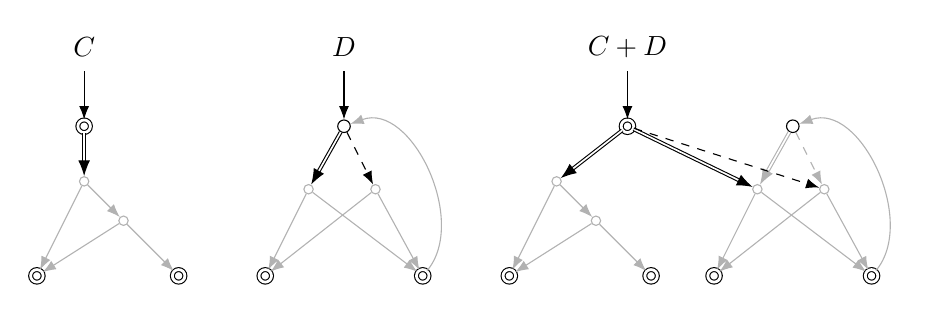
\begin{tikzpicture}[
  >=Latex,
  box/.style={rounded corners, draw, thick, inner sep=8pt, minimum width=2.3cm, minimum height=3cm},
  state/.style={circle, draw, inner sep=1.6pt},
  ghost/.style={circle, draw, inner sep=1.2pt, gray!60},
  final/.style={state, double, double distance=1pt},
  lab/.style={font=\small}
]

%------------ Boîte 1 (C1) -----------------
%\node[box] (B1) at (0,0) {};

% états (vertical compact)
\node (label) at (0,2) {$C$};
\node[final, label={[lab]left:$ $}] (i1) at (0,1.0) {};
\node[ghost] (q11) at (0,0.3) {};
\node[ghost] (q12) at (0.5,-0.2) {};
\node[final, label={[lab]below:$ $}]  (f11) at (-0.6,-0.9) {};
\node[final, label={[lab]below:$ $}] (f12) at (1.2,-0.9) {};

% transitions abstraites (patron 1)
\draw[->] (0,1.7) -- (i1.north);
%\draw[gray!60,->] (i1) -- (q11);
\draw[->, double] (i1) -- node[lab,right,pos=0.45] {$ $} (q11);
\draw[gray!60,->] (q11) to (q12);
\draw[gray!60,->] (q12) -- (f11);
\draw[gray!60,->] (q12) -- (f12);
\draw[gray!60,->] (q11) to (f11);

\begin{scope}[shift={(-.7,0)}]

\node[state, label={[lab]left:$ $}] (i2) at (4,1.0) {};
\node[ghost] (p21) at (3.55,0.2) {};
\node[ghost] (p22) at (4.4,0.2) {};
\node[final, label={[lab]below:$ $}]  (f21) at (3,-0.9) {};
\node[final, label={[lab]below:$ $}] (f22) at (5,-0.9) {};

\node (label) at (4,2) {$D$};
% transitions abstraites (patron 2)

\draw[->] (4,1.7) -- (i2.north);
\draw[->, double] (i2) -- node[lab,left,pos=0.45] {$ $} (p21);
\draw[->, dashed] (i2) -- node[lab,right,pos=0.45] {$ $} (p22);
\draw[gray!60,->] (p21) -- (f21);
\draw[gray!60,->] (p22) -- (f22);
\draw[gray!60,->] (p21) to (f22);
\draw[gray!60,->] (p22) to (f21);
\draw[gray!60,->] (f22) to[in = 20, out=50]  (i2);
\end{scope}
\begin{scope}[shift={(5,0)}]

%------------ Boîte 1 (C1) -----------------
%\node[box] (B1) at (0,0) {};

% états (vertical compact)
%\node[final, label={[lab]above:$ $}] (i1) at (0,1.0) {};

\begin{scope}[shift={(1,0)}]
\node[ghost] (q11a) at (0,0.3) {};
\node[ghost] (q12a) at (0.5,-0.2) {};
\node[final, label={[lab]below:$ $}]  (f11a) at (-0.6,-0.9) {};
\node[final, label={[lab]below:$ $}] (f12a) at (1.2,-0.9) {};

% transitions abstraites (patron 1)
%\draw[gray!60,->, double] (i1) -- (q11);
\draw[gray!60,->] (q11a) to (q12a);
\draw[gray!60,->] (q12a) -- (f11a);
\draw[gray!60,->] (q12a) -- (f12a);
\draw[gray!60,->] (q11a) to (f11a);
\end{scope}
%------------ Boîte 2 (C2) -----------------
%\node[box] (B2) at (6,0) {};

% états
\node[state, label={[lab]above:$ $}] (i2a) at (4,1.0) {};
\node[ghost] (p21a) at (3.55,0.2) {};
\node[ghost] (p22a) at (4.4,0.2) {};
\node[final, label={[lab]below:$ $}]  (f21a) at (3,-0.9) {};
\node[final, label={[lab]below:$ $}] (f22a) at (5,-0.9) {};


% transitions abstraites (patron 2)
\draw[gray!60,->, double] (i2a) -- (p21a);
\draw[gray!60,->, dashed] (i2a) -- (p22a);
\draw[gray!60,->] (p21a) -- (f21a);
\draw[gray!60,->] (p22a) -- (f22a);
\draw[gray!60,->] (p21a) to (f22a);
\draw[gray!60,->] (p22a) to (f21a);
\draw[gray!60,->] (f22a) to[in = 20, out=50] (i2a);

%------------ Nouvel état initial i (somme) --------------
\node (label) at (1.9,2) {$C + D$};
\node[final, label={[lab]right:$ $}] (inew) at (1.9,1.0) {}; % final car i1 est final
% flèche initiale globale
\draw[->] (1.9,1.7) -- (inew.north);

% Transitions de i vers les cibles des transitions de i1 et i2
% (elles reproduisent: (i,a,q) si (i1,a,q) ou (i2,a,q) étaient dans Δ1 ou Δ2)
\draw[->, double] (inew) -- node[lab,above,pos=0.55] {$ $} (q11a);
%\draw[->] (inew) -- node[lab,above,pos=0.55] {$b$} (q12);
\draw[->, double] (inew) -- node[lab,below,pos=0.45] {$ $} (p21a);
\draw[->, dashed] (inew) -- node[lab,above,pos=0.45] {$ $} (p22a);

\end{scope}

\end{tikzpicture}
\end{center}
\end{example}


% \begin{definition}
% For $i=1,2$, let $C_i = (Q_i, \Sigma, \Delta_i, I_i, F_i)$ be a chart. 
% \emph{Sequential composition} of $C_1$ and $C_2$, denoted $C_1 \cdot C_2$, is the chart  whose:
% \begin{itemize}
%     \item set of states is obtained from $Q_1 \sqcup Q_2$ by removing $I_2$ if $C_2$ is rooted,
%     \item initial state is $I_1$,
%     \item set of final states is $F_2$ to which we add $F_1$ if $I_2\in F_2$ and from which we
%      remove $I_2$ if $C_2$ is rooted.
%     \item  transition relation is obtained from $\Delta_1 \sqcup \Delta_2$ by removing the 
%     transitions involving the state $I_2$ if it has been removed, then adding:
%     $$\{\, (f,a,q) \mid f \in F_{1} \text{ and } (I_2,a,q) \in \Delta_{2} \,\}.$$
% \end{itemize}
% \end{definition}

\begin{definition}
The sequential composition $C_1 \cdot C_2$ of two charts $C_1$ and $C_2$ is 
the chart whose state set is the disjoint union of their state sets, 
removing the initial state $I_2$ of $C_2$ if that chart was rooted. 
Its initial state is that of $C_1$. Its final states are those of $F_2$,
 together with the finals of $C_1$ if $I_2$ was final, and minus $I_2$ if it was removed.
 The derivatives of the states are inherited from $C_1$ and $C_2$, except for the final states of 
 $C_1$ to which we add the derivatives of $I_2$.
\end{definition}
\begin{example} The sequential composition if two charts $C$ and $D$ where $D$ is rooted.
    \begin{center}
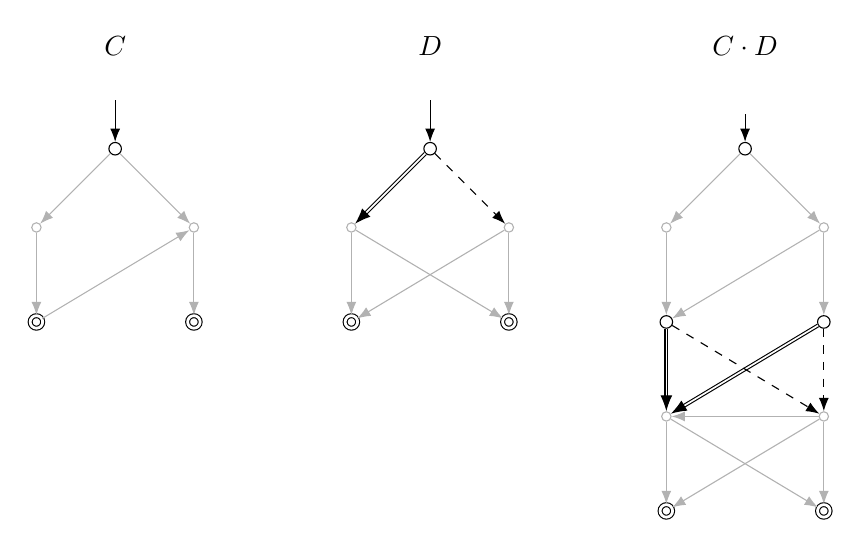
\begin{tikzpicture}[
  >=Latex,
  state/.style={circle, draw, inner sep=1.6pt},
  ghost/.style={circle, draw, inner sep=1.2pt, gray!60},
  final/.style={state, double, double distance=1pt},
  lab/.style={font=\small},
  every edge quotes/.style={auto, text=black, font=\small}
]

% ======================= C1 (gauche->droite) =======================
\begin{scope}[shift={(-6,0)},rotate=-90]
  \node (labC1) at (-2.5,0) {$C$};

  % états C1
  \node[state] (i1) at (-1.2,0) {};
  \node[ghost] (x1) at (-0.2,1) {};
  \node[ghost] (x2) at (-0.2,-1) {};
  \node[final] (f1) at (1.0,1) {};
  \node[final] (f1p) at (1.0,-1) {};

  % flèche initiale
  \draw[->] ([xshift=-15pt]i1.north) -- (i1.north);

  % transitions internes (gris)
  \draw[gray!60,->] (i1) -- (x1);
  \draw[gray!60,->] (i1) -- (x2);
  \draw[gray!60,->] (x1) -- (f1);
  \draw[gray!60,->] (x2) -- (f1p);
  \draw[gray!60,->] (f1p) to (x1);
\end{scope}

% ======================= C2 (gauche->droite) =======================
\begin{scope}[shift={(-2,0)}, ,rotate=-90]
  \node (labC2) at (-2.5,0) {$D$};

  % états C2
  \node[state] (i2) at (-1.2,0) {};
  \node[ghost] (y1) at (-0.2,1) {};
  \node[ghost] (y2) at (-0.2,-1) {};
  \node[final] (g1) at (1.0,1) {};
  \node[final] (g2) at (1.0,-1) {};

  % flèche initiale
  \draw[->] ([xshift=-15pt]i2.north) -- (i2.north);

  % sorties explicites de i2
  \draw[->, dashed] (i2) -- (y1) node[midway,above,lab] {$ $};
  \draw[->, double] (i2) -- (y2) node[midway,below,lab] {$ $};

  % transitions internes (gris)
  \draw[gray!60,->] (y1) -- (g1);
  \draw[gray!60,->] (y2) -- (g2);
  \draw[gray!60,->] (y1) to (g2);
  \draw[gray!60,->] (y2) to (g1);
\end{scope}
\begin{scope}[shift={(2,0)}, rotate=-90]
    \node (labSeq) at (-2.5,0) {$C \cdot D$};

% copie visuelle de C1 (à gauche)
\node[state] (i1s) at (-1.2,0) {};
\node[ghost] (xs1) at (-0.2,1) {};
\node[ghost] (xs2) at (-0.2,-1) {};
\node[state] (fs1) at (1.0,1) {};
\node[state] (fs2) at (1.0,-1) {};


% copie visuelle de C2 (à droite)
%\node[state] (i2s) at (1.0,0) {}; % i2 lui-même n'est pas final
\node[ghost] (ys1) at (2.2,1) {};
\node[ghost] (ys2) at (2.2,-1) {};
\node[final] (gs1) at (3.4,1) {};
\node[final] (gs2) at (3.4,-1) {};

% flèche initiale globale: i1
\draw[->] ([xshift=-10pt]i1s.north) -- (i1s.north);

% Δ1 (gris)
\draw[gray!60,->] (i1s) -- (xs1);
\draw[gray!60,->] (i1s) -- (xs2);
\draw[gray!60,->] (xs1) -- (fs1);
\draw[gray!60,->] (xs2) -- (fs2);
\draw[gray!60,->] (xs1) to (fs2);

% Δ2 (gris)
%\draw[gray!60,->, dashed] (i2s) -- (ys1);
%\draw[gray!60, ->, double] (i2s) -- (ys2);
\draw[gray!60,->] (ys1) -- (gs1);
\draw[gray!60,->] (ys1) -- (ys2);
\draw[gray!60,->] (ys2) -- (gs2);
\draw[gray!60,->] (ys1) to (gs2);
\draw[gray!60,->] (ys2) to (gs1);

% Règle de concaténation: copier sorties de i2 sur chaque f∈F1
% Utilisation de bend pour éviter croisements
\draw[->, dashed] (fs1) to[bend left=0] node[lab,above] {$ $} (ys1);
\draw[->, double] (fs1) to[bend left=0] node[lab,below] {$ $} (ys2);

\draw[->, dashed] (fs2) to[bend right=0] node[lab,below] {$ $} (ys1);
\draw[->, double] (fs2) to[bend right=0] node[lab,above] {$ $} (ys2);

\end{scope}
\end{tikzpicture}
\end{center}
\end{example}

%\begin{definition}
%     Let $C = (Q, \Sigma, \Delta, I, F)$ be a chart. The \emph{star} of $C$, denoted $C^*$, is the chart whose:
%     \begin{itemize}
%         \item set of states is $Q$ to which we add a fresh state $I'$ and remove $I$ if 
%         $C$ is rooted,
%         \item initial state is $I'$,
%         \item set of final states is $F$ to which we add $I'$ and remove $I$ if $C$ is rooted,
%         \item transition relation is obtained from $\Delta$ by removing the transitions involving $I$ 
%         if it has been removed, then adding:
%         $$\{ (p, a, q) \mid p \in F\cup \{I'\},\ (I, a, q) \in \Delta \}.$$
%     \end{itemize}
% \end{definition}

\begin{definition}
The star $C^{*}$ of a chart $C$ is the chart obtained as follows. 
Its set of states is that of $C$, plus a fresh initial state $I'$, and minus the old initial state $I$ if $C$ was rooted. 
The new initial state is $I'$. 
The set of final states consists of the finals of $C$ together with $I'$, with $I$ removed if it was deleted. 
The transition relation is inherited from $C$, except that each final state of $C$ additionally inherits all outgoing transitions of $I$; moreover, $I'$ has exactly the outgoing transitions of $I$.
\end{definition}


\begin{example} Let $C$ be a the left chart, it ietaration $C^*$ is the right chart. 
\begin{center}
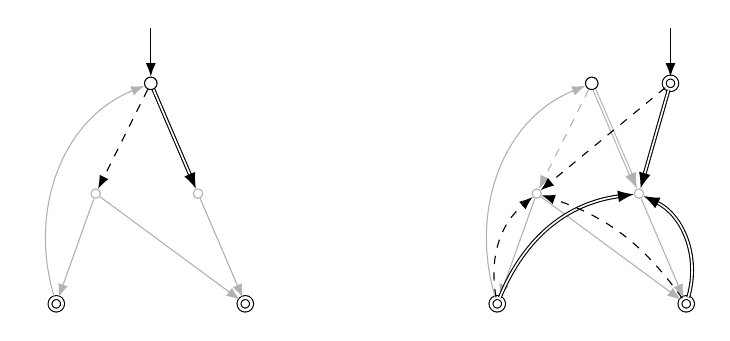
\begin{tikzpicture}[
  >=Latex,
  state/.style={circle, draw, inner sep=1.6pt},
  ghost/.style={circle, draw, inner sep=1.2pt, gray!60},
  final/.style={state, double, double distance=1pt},
  lab/.style={font=\small},
  every edge quotes/.style={auto, text=black, font=\small}
]

% ======================= C (vertical) =======================
\begin{scope}[shift={(-2.8,0)}]
  %\node (labC) at (0,2.3) {$C$};

  % états C
  \node[state] (i1) at (0,1.4) {};
  \node[ghost] (q1) at (-0.7,-0) {};
  \node[ghost] (q2) at ( 0.6,-0) {};
  \node[final] (f1) at (-1.2,-1.4) {};
  \node[final] (f2) at ( 1.2,-1.4) {};

  % flèche initiale
  \draw[->] (0,2.1) -- (i1.north);

  % sorties explicites de i1
  \draw[->, dashed] (i1) -- (q1);
  \draw[ ->, double ] (i1) -- (q2);

  % transitions internes (gris)
  \draw[gray!60,->] (q1) to (f1);
  \draw[gray!60,->] (q2) to (f2);
  \draw[gray!60,->] (q1) to (f2);
  \draw[gray!60,->] (f1) to[bend left, in=135, out =40]  (i1);
\end{scope}

% ======================= C* (vertical) =======================
\begin{scope}[shift={(2.8,0)}]
  %\node (labS) at (0,2.8) {$C^{\!*}$};

  % nouvel initial i (final aussi)
  \node[final] (i)  at (1,1.4) {};

  \node[state] (i1s) at (0,1.4) {};
  \node[ghost] (r1) at (-0.7,-0) {};
  \node[ghost] (r2) at ( 0.6,-0) {};
  \node[final] (g1) at (-1.2,-1.4) {};
  \node[final] (g2) at ( 1.2,-1.4) {};


  % flèche initiale globale
  \draw[->] (1,2.1) -- (i.north);

  % Δ (gris) : transitions internes de C conservées
  \draw[gray!60,->, dashed] (i1s) -- (r1);
  \draw[gray!60,->, double] (i1s) -- (r2);
    \draw[dashed,->] (i) -- (r1);
  \draw[double , ->] (i) -- (r2);
  \draw[gray!60,->] (r1)  to (g1);
  \draw[gray!60,->] (r2)  to  (g2);
  \draw[gray!60,->] (r1)  to  (g2);
  \draw[gray!60,->] (g1)  to[bend left, in=135, out =40]  (i1s);
  % Ajouts pour l'étoile :
  % 1) Depuis i, recopier les sorties de i1
 % \draw[->] (i) to node[midway,above,lab] {$ $} (r1);
  %\draw[->, dashed] (i) to node[midway,above,lab] {$$} (r2);

  % 2) Depuis chaque f \in F, recopier les sorties de i1 (itération)
  %    ici F = {g1, g2}
  \draw[->, dashed ] (g1) to[bend left=30]  node[midway,left,lab]  {$ $} (r1);
\draw[->, double ] (g1) to[bend left=30] node[midway,above,lab] {$ $} (r2);


\draw[->, dashed]
    (g2) to[bend right=18] node[midway,right,lab] {$ $} (r1);
\draw[->, double]
    (g2) to[bend right=40] node[midway,above,lab] {$ $} (r2);
\end{scope}

\end{tikzpicture}
\end{center}
\end{example}
\begin{definition}
The \emph{Milner chart} $M(e)$ of a regular expression $e$ is defined inductively as follows:
\begin{itemize}
        \item $M(0) = (\{i, f\}, i, \{f\}, \emptyset)$
    \item $M(1) = (\{\star\}, \star, \{\star\}, \emptyset)$,
    \item $M(a) = (\{i, f\}, i, \{f\}, \{(i, a, f)\})$, 
    \item $M(e+f) = M(e) + M(f)$,
    \item $M(e \cdot f) = M(e) \cdot M(f)$,
    \item $M(e^*) = M(e)^*$.
\end{itemize}
\end{definition}

\begin{example} The milner chart of $a(b+c), (a(b+c))^*$ et $ab^*+c^*$.
\end{example}

\begin{proposition}
For every regular expression $e$, $M(e)$ is rooted.
\end{proposition}

\subsection{Bisimulation}
\begin{notation}
    If $C$ is a chart, we denote by $\xlongrightarrow{a}_{C}$ the relation on its set of states defined as:
    $$\xlongrightarrow{a}_{C} \;=\; \{ (p,q) \mid (p,a,q) \text{ is a transition of } C \}.$$
    We denote by $\xlongleftarrow{a}_{C}$ the converse of $\xlongrightarrow{a}_{C}$.
\end{notation}

\begin{definition}
Let $C$ and $D$ be two charts with state sets $Q$ and $Q'$ and respectively. A relation $R\subseteq Q\times Q'$ is a \emph{bisimulation} between $C$ and $D$ if:
\begin{itemize}
    \item $\forall (p,q)\in R$, $p$ is final $\; \Leftrightarrow\;$ $q$ is final,
    \item $\xlongleftarrow{a}_{C}\cdot R\ =\ R \cdot \xlongleftarrow{a}_{D}$ $\quad$ and $\quad$ $ \xlongrightarrow{a}_{C} \cdot R\;=\;R \cdot \xlongrightarrow{a}_{D}$.
\end{itemize}

Let $(p,q)\in C\times D$. We say that $p$ and $q$ are \emph{bisimilar}, and write $p\sim q$, if $(p,q)\in R$ for some bisimilation $R$ between $C$  and $D$.\\

We say that $C$ and $D$ are \emph{bisimilar}, and write $C \sim D$, if there initial states are bisimilar.
\end{definition}

\begin{definition}
The \emph{chart language} $\mathcal{C}(e)$ of a regular expression $e$ is the set of charts bisimilar to its Milner chart. 
\end{definition}

\subsection{Milner's Axiomatization}


\begin{definition} We define the \emph{finality} function $f$ from regular
         expressions to $\{0,1\}$
         as follows:
\[
\begin{aligned}
&f(0)=0, \quad f(1)=1, \quad f(a)=0 \quad (a \in \Sigma), \\[0.3em]
&f(e+g)=\max(f(e),f(g)), \quad f(eg)=f(e)f(g), \quad f(e^*)=1 .
\end{aligned}
\]
If $f(e)=1$ we write $e\Downarrow$ and say that $e$ is \emph{final}. Otherwise we write $e\Uparrow$. 
    \end{definition}




\begin{definition} \emph{Milner's proof system} 
    contains the following axioms and deduction rules:~\\
    
\textbf{Algebraic laws:}
\[
\renewcommand{\arraystretch}{1.6} % espace vertical entre lignes
\begin{array}{@{\hspace{3pt}}r@{\hspace{6pt}}l
                  @{\hspace{25pt}}r@{\hspace{6pt}}l
                  @{\hspace{25pt}}r@{\hspace{6pt}}l}
\text{\scriptsize (1)}  & e + f = f + e            
  & \text{\scriptsize (5)}  & (ef)g = e(fg)         
  & \text{\scriptsize (9)}  & e + 0 = e \\

\text{\scriptsize (2)}  & (e + f) + g = e + (f + g) 
  & \text{\scriptsize (6)}  & 1e = e = e1           
  & \text{\scriptsize (10)} & 0e = 0 = e0 \\

\text{\scriptsize (3)}  & e + e = e                 
  & \text{\scriptsize (7)}  & (e+f)g = eg + fg      
  & \text{\scriptsize (11)} & 0^* = 1 \\

\text{\scriptsize (4)}  & e^* = 1 + e e^*           
  & \text{\scriptsize (8)}  & e^* = (e+1)^*         
  &                     & 
\end{array}
\]

\textbf{Salooma's induction rule:}
\vspace{.5em}
\[
\frac{\, f= ef + g\qquad e\Uparrow\,}{\,f=e^*g\,}
\]

\textbf{Congruence rules:}
\[
\renewcommand{\arraystretch}{1.8}
\begin{array}{c@{\hspace{35pt}}c@{\hspace{35pt}}c}
\dfrac{}{\,e = e\,} 
  & \dfrac{\,e = f\,}{\,f = e\,} 
  & \dfrac{\,e = f \;\; f = h\,}{\,e = h\,} \\[12pt]
\dfrac{\,e_1 = f_1 \;\; e_2 = f_2\,}{\,e_1 + e_2 = f_1 + f_2\,}
  & \dfrac{\,e_1 = f_1 \;\; e_2 = f_2\,}{\,e_1 e_2 = f_1 e_2\,}
  & \dfrac{\,e = f\,}{\,e^{*} = f^{*}\,}
\end{array}
\]
\vspace{1em}

We say that two regular expressions $e$ and $f$ are \emph{provably equivalent} in the Milner system, denoted $e \equiv f$, if the equation $e = f$ is derivable from the axioms (1-11), Salomaa's  rule and congruence rules.
\end{definition}



\section{Rewriting system for charts}



    \begin{definition} We consider the following rewriting rules,  which transform charts over $\Sigma^*$ into charts
         over
         $\Sigma^*$. They are to be interpreted as follows:
              squares represent states for which some transitions are depicted but not necessarily all of them.
               Circles represent states with all transitions explicitly shown.
                    Circles are distinct from surrounding nodes, unlike squares. 

         \begin{itemize}
          \item \textbf{Zero rule:}~\\
            \begin{center}
        \begin{tikzpicture}[node distance=1.8cm, scale=1.0, every node/.style={transform shape}]
            % Left side (before)
            \node[state] (p1) at (0,0) {};
            \node[state] (q1) at (0,-1.8) {};      
            % Arrow between rules
            \node (i) at (2,-0.9) {$\twoheadrightarrow_{\mathsf{0}}$};
            %\node[below=1.2cm of i] {Zero rule};
            % Right side (after)
            \node[state] (p2) at (4,0) {};
            \node[state] (q2) at (4,-1.8) {};
            \draw[arr] (p2) to node[right] {$0$} (q2);  
        \end{tikzpicture}~\\
            \end{center}
            \item \textbf{Parallel transitions merge:}~\\
            \begin{center}
                    \begin{tikzpicture}[node distance=1.8cm, scale=1.0, every node/.style={transform shape}]
            % Left side (before)
            \node[state] (p1) at (0,0) {};
            \node[state] (q1) at (0,-1.8) {};
            \draw[arr] (p1) to[bend left=20] node[right] {$f$} (q1);
            \draw[arr] (p1) to[bend right=20] node[left]  {$e$} (q1);

            % Arrow between rules
            \node (i) at (2,-0.9) {$\twoheadrightarrow_{\mathsf{p}}$};
           % \node[below=1.2cm of i] {Transitions fusion};
        
            % Right side (after)
            \node[state] (p2) at (4,0) {};
            \node[state] (q2) at (4,-1.8) {};
            \draw[arr] (p2) to node[right] {$e+f$} (q2);
        \end{tikzpicture}~\\
            \end{center}
    % \item \textbf{Loopless state elimination} (the circle state is not initial, nor final):~\\
    % \begin{center}
    %  \begin{tikzpicture}[node distance=1.8cm, scale=1.0, every node/.style={transform shape}]
    %         % Left side (before)
    %         \node[state] (p1) at (4,0) {};
    %         \node (d1) at (4.5,0) {$\dots$};
    %         \node[state] (q1) at (5,0) {};
    %         \node[circ] (r1) at (4.5,-1.2) {};
    %         \node[state] (s1) at (4.5,-2.4) {};
    %         \draw[arr] (p1) to node[left] {$e_1$} (r1);
    %         \draw[arr] (q1) to node[right] {$e_n$} (r1);
    %         \draw[arr] (r1) to node[right] {$f$} (s1);
    %         \node (d1') at (4.5,-.6) {\tiny $\dots$};
    %         % Arrow between rules
    %         \node (i) at (6.5,-1.2) {$\twoheadrightarrow_{\mathsf{d}}$};
    %         %\node[below=2cm of i] {Loopless state elimination};

    %         % Right side (after)
    %         \pgfmathsetmacro{\shift}{8}
    %         \node[state] (p2) at (\shift,0) {};
    %         \node[state] (q2) at (\shift+1,0) {};
    %         \node[state] (s2) at (\shift+0.5,-2.4) {};
    %         \draw[arr] (p2) to node[left] {$e_1f$} (s2);
    %         \draw[arr] (q2) to node[right] {$e_nf$} (s2);
    %         \node (d2) at (\shift+0.5,0) {$\dots$};
    %         \node (d2') at (\shift+0.5,-1.2) {{\tiny $\dots$}};
    %     \end{tikzpicture}\\
    % \end{center}
       \item \textbf{State elimination} (the circle state is not initial, nor final):\\
        \begin{center}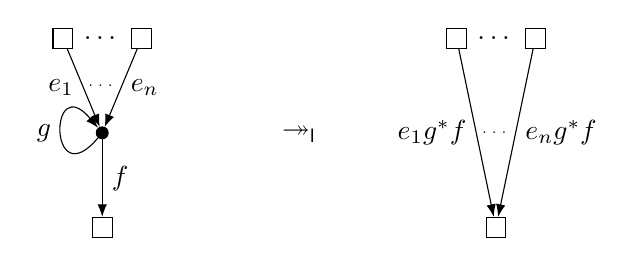
\begin{tikzpicture}[node distance=1.8cm, scale=1.0, every node/.style={transform shape}]
            % Left side (before)
            \node[state] (p1) at (6,0) {};
            \node (d1) at (6.5,0) {$\dots$};
            \node[state] (q1) at (7,0) {};
            \node[circ] (r1) at (6.5,-1.2) {};
            \node[state] (s1) at (6.5,-2.4) {};
            \draw[arr] (p1) to node[left] {$e_1$} (r1);
            \draw[arr] (q1) to node[right] {$e_n$} (r1);
            \draw[arr] (r1) to node[right] {$f$} (s1);
            \draw[arr] (r1) to[loop left, looseness=20, out=-130, in=130] node[left] {$g$} (r1);
            \node (d1') at (6.5,-.6) {\tiny $\dots$};
            % Arrow between rules
            \node (i) at (9,-1.2) {$\twoheadrightarrow_\mathsf{l}$};
            %\node[below=2cm of i] {Safe loop elimination ($g\Uparrow$ only)};

            % Right side (after)
            \pgfmathsetmacro{\shift}{11}
            \node[state] (p2) at (\shift,0) {};
            \node[state] (q2) at (\shift+1,0) {};
            \node[state] (s2) at (\shift+0.5,-2.4) {};
            \draw[arr] (p2) to node[left] {$e_1g^*f$} (s2);
            \draw[arr] (q2) to node[right] {$e_ng^*f$} (s2);
            \node (d2) at (\shift+0.5,0) {$\dots$};
            \node (d2') at (\shift+0.5,-1.2) {{\tiny $\dots$}};
        \end{tikzpicture}\\
    \end{center}
    \item \textbf{Renaming} (when $e \equiv f$): \\
    \begin{center}
        \begin{tikzpicture}[node distance=1.8cm, scale=1.0, every node/.style={transform shape}]
            % Left side (before)
            \node[state] (p1) at (0,0) {};
            \node[state] (q1) at (0,-1.8) {};  

            \draw[arr] (p1) to node[right] {$e$} (q1);
            % Arrow between rules
            \node (i) at (2,-0.9) {$\twoheadrightarrow_{\mathsf{r}}$};
            %\node[below=1.2cm of i] {Renaming};
            % Right side (after)
            \node[state] (p2) at (4,0) {};
            \node[state] (q2) at (4,-1.8) {};
            \draw[arr] (p2) to node[right] {$f$} (q2);  
        \end{tikzpicture}~\\
            \end{center}
    \item \textbf{Factorization} :\\
    \begin{center}
          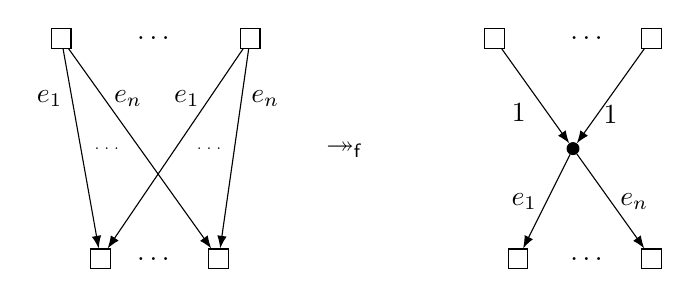
\begin{tikzpicture}[scale=1.0, every node/.style={transform shape}]
            % Left side (before)

            \begin{scope}[shift={(-.5,0)}]
          %  \node[] (p1) at (0.5,0.5) {$p_1$};
            \node[state] (p1) at (0.5,0) {};
               \node[state] (pn) at (2.9,0) {};
            \node[state] (q1) at (1,-2.8) {};
            \node[state] (q2) at (2.5,-2.8) {};
            \node (dots) at (1.7,-2.8) {$\dots$};
            \node (dots) at (1.7,0) {$\dots$};
            \node (ad) at (1.1,-1.4) {\tiny $\dots$};
            \node (ad) at (2.4,-1.4) {\tiny $\dots$};
            \draw[arr] (p1) to node[left, near start] {$e_1$} (q1);
            \draw[arr] (p1) to node[right, near start] {$e_n$} (q2);
            \draw[arr] (pn) to node[left, near start] {$e_1$} (q1);
            \draw[arr] (pn) to node[right, near start] {$e_n$} (q2);
            \end{scope}
            % Arrow between rules
            \node (i) at (3.6,-1.4) {$\twoheadrightarrow_{\mathsf{f}}$};
           % \node[below=1.4cm of i] {Factorization};

            % Right side (after)
            % \pgfmathsetmacro{\shift}{.5}
            \begin{scope}[shift={(5,0)}]
                \node[state] (sp1) at (.5,0) {};
                \node[state] (spn) at (2.5,0) {};
                \node[state] (sq1) at (0.8,-2.8) {};
                \node[state] (sq2) at (2.5,-2.8) {};
                \node[circ] (c) at (1.5,-1.4) {};
                \node (sdots) at (1.7,-2.8) {$\dots$};
            \node (sdots) at (1.7,0) {$\dots$};
            \draw[arr] (c) to node[left] {$e_1$} (sq1);
            \draw[arr] (c) to node[right] {$e_n$} (sq2);
            \draw[arr] (sp1) to node[left, yshift=-6pt, midway ] {$1$} (c);
            \draw[arr] (spn) to node[right, below ] {$1$} (c);
            \end{scope}
        \end{tikzpicture}\\
    \end{center}
    \end{itemize}
    We let $\twoheadrightarrow$ denote the union of all these rewriting rules.
    \end{definition}
    \begin{remark}
   If in a chart, some states $q_1,\dots, q_m $ have a common subset
     $S$ of derivatives, then the rewriting rule 
    $\twoheadrightarrow_{\mathsf{f}}$:
    \begin{itemize}
    \item creates a fresh state $q$ such that $D(q)=S$,
    \item removes $S$ from the derivatives of $q_i$ and adds $(1,q)$, for $i\in\{1,\dots,m\}$.
    \end{itemize}
    %We call the states $q_1,\dots, q_n$ \emph{partners} and $q$ their \emph{factor}.
    \end{remark}
    % We denote by:
    % \begin{itemize}
    %     \item $\twoheadrightarrow$ the union of the above rewriting rules.
    %     \item $\twoheadrightarrow_{\mathsf{c}}$ the union of all these rewriting rules except the 
    %     factorisation rule.
    %     \item $\twoheadrightarrow_{\mathsf{s}}$ the factorization rule where the partners are pairwise
    %     co-accessible.\footnote{Voici un moyen mnemothéchnique pour se souvenir des differentes noms de règles:
    %     $\mathsf{p}$ stands for parallel transitions fusion, $\mathsf{d}$ stands for 
    %     distribution (this rule is very closed to the distributivity rule as we will see later), 
    %     $\mathsf{l}$ stands for loop elimination, $\mathsf{f}$ stands for factorization, $\mathsf{c}$ stands for classical rules and $\mathsf{s}$ stands for strong factorization rule.}
    % \end{itemize}
   
    % 
        %          A chart  \emph{reducible} if it can be rewritten by $\twoheadrightarrow^*$ until no 
        %          inner state remains.
        %          
        %          into a chart of the
        %          form:
        % \begin{center}
        %     \begin{tikzpicture}[
        %   >=Latex,
        %   state/.style={circle, draw, inner sep=1.6pt},
        %   ghost/.style={circle, draw, inner sep=1.2pt, gray!60},
        %   final/.style={state, double, double distance=1pt},
        %   lab/.style={font=\small},
        %   every edge quotes/.style={auto, text=black, font=\small}
        % ]
        %
        %         % First chart
        %         \node[circ] (p1) at (0,0) {};
        %         \node[final] (f1) at (2,0) {};
        %         \draw[arr] (p1) to node[above] {$e$} (f1);
        %         % Incoming and outgoing arrows (horizontal)
        %         \draw[arr] ([xshift=-5mm]p1.west) to (p1);
        %     \end{tikzpicture}
        % \end{center}
     
        
        %         \begin{figure}[h!]
        %     \begin{flushleft}
        %         \scalebox{1}{ 
        %     \begin{tabular}[t]{@{}c@{\hspace{1.4cm}}c@{}}
        %         \begin{tikzpicture}[node distance=1.8cm, scale=1.0, every node/.style={transform shape}]
        %             % Left side (before)
        %             \node[state] (p1) at (0,0) {};
        %             \node[state] (q1) at (0,-1.8) {};
        %             \draw[arr] (p1) to[bend left=20] node[right] {$f$} (q1);
        %             \draw[arr] (p1) to[bend right=20] node[left]  {$e$} (q1);
        %
        %             % Arrow between rules
        %             \node (i) at (1,-0.9) {$\twoheadrightarrow$};
        %             \node[below=1.2cm of i] {Transitions fusion};
        %         
        %             % Right side (after)
        %             \node[state] (p2) at (2,0) {};
        %             \node[state] (q2) at (2,-1.8) {};
        %             \draw[arr] (p2) to node[right] {$e+f$} (q2);
        %
        %         \end{tikzpicture}
        %         &
        %            \begin{tikzpicture}[node distance=1.8cm, scale=1.0, every node/.style={transform shape}]
        %             % Left side (before)
        %             \node[state] (p1) at (0,0) {};
        %             \node[state] (q1) at (0,-1.8) {};
        %
        %             % Arrow between rules
        %             \node (i) at (.7,-0.9) {$\twoheadrightarrow$};
        %             \node[below=1.2cm of i] {Zero rule};
        %         
        %             % Right side (after)
        %             \node[state] (p2) at (1.4,0) {};
        %             \node[state] (q2) at (1.4,-1.8) {};
        %             \draw[arr] (p2) to node[right] {$0$} (q2);
        %
        %         \end{tikzpicture}\\[1.5cm]
        %         % Elimination rule
        %         \begin{tikzpicture}[node distance=1.8cm, scale=1.0, every node/.style={transform shape}]
        %             % Left side (before)
        %             \node[state] (p1) at (4,0) {};
        %             \node (d1) at (4.5,0) {$\dots$};
        %             \node[state] (q1) at (5,0) {};
        %             \node[circ] (r1) at (4.5,-1.2) {};
        %             \node[state] (s1) at (4.5,-2.4) {};
        %             \draw[arr] (p1) to node[left] {$e_1$} (r1);
        %             \draw[arr] (q1) to node[right] {$e_n$} (r1);
        %             \draw[arr] (r1) to node[right] {$f$} (s1);
        %             \node (d1') at (4.5,-.6) {\tiny $\dots$};
        %             % Arrow between rules
        %             \node (i) at (5.5,-1.2) {$\twoheadrightarrow$};
        %             \node[below=2cm of i] {Loopless state elimination};
        %
        %             % Right side (after)
        %             \pgfmathsetmacro{\shift}{6.5}
        %             \node[state] (p2) at (\shift,0) {};
        %             \node[state] (q2) at (\shift+1,0) {};
        %             \node[state] (s2) at (\shift+0.5,-2.4) {};
        %             \draw[arr] (p2) to node[left] {$e_1f$} (s2);
        %             \draw[arr] (q2) to node[right] {$e_nf$} (s2);
        %             \node (d2) at (\shift+0.5,0) {$\dots$};
        %             \node (d2') at (\shift+0.5,-1.2) {{\tiny $\dots$}};
        %         \end{tikzpicture}
        %         &
        %         % Elimination rule
        %
        %     \end{tabular}}
        % \end{flushleft}
        % ~\\[.5cm]
        %     % Factorization rule
        % \begin{center}
        %   \begin{tikzpicture}[scale=1.0, every node/.style={transform shape}]
        %             % Left side (before)
        %             \node[state] (p1) at (-.5,0) {};
        %                \node[state] (pn) at (3.5,0) {};
        %             \node[state] (q1) at (1,-2.8) {};
        %             \node[state] (q2) at (2.5,-2.8) {};
        %             \node (dots) at (1.7,-2.8) {$\dots$};
        %             \node (dots) at (1.7,0) {$\dots$};
        %             \node (ad) at (.7,-1.4) {\tiny $\dots$};
        %             \node (ad) at (2.7,-1.4) {\tiny $\dots$};
        %             \draw[arr] (p1) to node[left] {$e_1$} (q1);
        %             \draw[arr] (p1) to node[right] {$e_n$} (q2);
        %             \draw[arr] (pn) to node[left] {$e_1$} (q1);
        %             \draw[arr] (pn) to node[right] {$e_n$} (q2);
        %
        %             % Arrow between rules
        %             \node (i) at (5,-1.4) {$\twoheadrightarrow$};
        %             \node[below=1.4cm of i] {Factorization};
        %
        %             % Right side (after)
        %             % \pgfmathsetmacro{\shift}{.5}
        %             \begin{scope}[shift={(7,0)}]
        %                 \node[state] (sp1) at (-.5,0) {};
        %                 \node[state] (spn) at (3.5,0) {};
        %                 \node[state] (sq1) at (0.8,-2.8) {};
        %                 \node[state] (sq2) at (2.5,-2.8) {};
        %                 \node[circ] (c) at (1.5,-1.4) {};
        %                 \node (sdots) at (1.7,-2.8) {$\dots$};
        %             \node (sdots) at (1.7,0) {$\dots$};
        %             \draw[arr] (c) to node[left] {$e_1$} (sq1);
        %             \draw[arr] (c) to node[right] {$e_n$} (sq2);
        %             \draw[arr] (sp1) to node[left, below ] {$1$} (c);
        %             \draw[arr] (spn) to node[right, below ] {$1$} (c);
        %             \end{scope}
        %         \end{tikzpicture}
        %     \end{center}
        %   
        %     \caption{The rules are interpreted as follows.
        %      Squares represent states for which some transitions are depicted but not necessarily all of them.
        %         Circles represent states with all transitions explicitly shown.
        %             Circles are distinct from surrounding nodes, unlike squares. The elimination rules do not remove the initial, nor a final state.
        %             The factorization rule introduces a new state.}   \label{fig:chart-rewriting-rules}
        % \end{figure}

~\\
As in the classical state-elimination algorithm, we apply the rewriting system only to charts that are rooted and terminal (i.e., with a unique sink final state). If a chart does not meet these conditions, we first normalise it by applying a \emph{root extension} and/or a \emph{sink completion}, defined below.

\begin{definition}
     \emph{Root extension} is the operation of adding a fresh state to a chart which becomes its new inital state,
     the adding a $1$-labelled transition from this state to the old initial state.

    \emph{Sink completion} is the operation of adding a fresh state to a chart, which becomes its unique final state, 
    and adding a $1$-labelled transition from every old final state to the new one.

     \emph{Normalisation} is the operation of root extension and sink completion. We denote by 
     $\llbracket C \rrbracket$ the normal form of a chart $C$.
\end{definition}

\begin{definition}
For every regular expressions $e$, we let ${N}(e)$ be the chart:
\begin{center}
        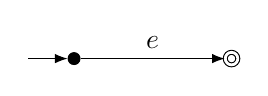
\begin{tikzpicture}[
      >=Latex,
      state/.style={circle, draw, inner sep=1.6pt},
      ghost/.style={circle, draw, inner sep=1.2pt, gray!60},
      final/.style={state, double, double distance=1pt},
      lab/.style={font=\small},
      every edge quotes/.style={auto, text=black, font=\small}
    ]

            % First chart
            \node[circ] (p1) at (0,0) {};
            \node[final] (f1) at (2,0) {};
            \draw[arr] (p1) to node[above] {$e$} (f1);
            % Incoming and outgoing arrows (horizontal)
            \draw[arr] ([xshift=-5mm]p1.west) to (p1);
        \end{tikzpicture}
    \end{center}
\end{definition}

\begin{definition}
    A chart $C$ is \emph{reducible} if there is a regular expression $e$ where:
     $$\llbracket C\rrbracket \twoheadrightarrow^* N(e).$$
\end{definition}

\begin{definition}
    A regular expression is \emph{safe} if in every sub-expression of the form $f^*$, we have $f\Uparrow$.
\end{definition}

\begin{proposition}
  Every expression is equivalent to a safe one.
    ~\label{prop:every-expression-is-equivalent-to-a-safe-one}
\end{proposition}

\begin{proposition} For every safe expression $e$, $M(e)$ is reducible.
    ~\label{prop:Milner-is-reducible}
\end{proposition}

\begin{example}
    Sur l'utilité de la restriction à one outgoing edge: $M(a(b+c))$, commentaire sur la règle $\twoheadrightarrow_{\mathsf{d}}$.
     Si on n'avait pas la restriction à one outgoing edge, on pourrait réduire mais ça ne serait pas 
     la bonne sémantique.

    Sur l'utilité de la factorization. Cette restriction est trop forte. Par exemple on ne pourra pas
    réduire $M((a(b+c))^*)$ sans la règle de factorisation.

    Toutes les chartes ne sont pas réductibles. Donner un exemple bisimilaire a une Milner chart, et un autre pas.
\end{example}



% \subsection{Properties of the rewriting rule system}

% \begin{definition}
% Let $C$ be a chart. The chart $R_n(C)$ is obtained from $C$ 
% by adding $n$ fresh states $I_1, \dots, I_n$ whose derivatives are those of $I$. 
%  We say that $R_n(C)$ is the  \emph{$n$ root extension} of $C$.
% \end{definition}

% \begin{lemma}
%     If $C$ reduce to $N(e)$ then $R_n(C)$ reduces to the following chart:
%         \begin{center}
%         \begin{tikzpicture}[
%       >=Latex,
%       state/.style={circle, draw, inner sep=1.6pt},
%       ghost/.style={circle, draw, inner sep=1.2pt, gray!60},
%       final/.style={state, double, double distance=1pt},
%       lab/.style={font=\small},
%       every edge quotes/.style={auto, text=black, font=\small}
%     ]

%             % First chart
%             \node[circ] (p1) at (-1.5,0) {};
%             \node[circ] (I1) at (-1.2,1) {};
%             \node[circ] (In) at (0,1.5) {};
%             \node[final] (f1) at (0,0) {};
%             \draw[arr] (I1) to node[above, midway] {$e$} (f1);
%             \draw[arr] (In) to node[right, midway] {$e$} (f1);
%             \draw[arr] (p1) to node[above , midway] {$e$} (f1);
%             % Incoming and outgoing arrows (horizontal)
%             \draw[arr] ([xshift=-5mm]p1.west) to (p1);
%         \end{tikzpicture}
%     \end{center}
% \end{lemma}

% \subsection{ Milner chart of a regular expression is reducible}


% \begin{lemma}\label{prop:Milner-is-reducible}For every regular expression $e$,
%      there is a regular expression $f$ such that $e\equiv f$ and:
%      $$\underline{M}(e)\twoheadrightarrow^*
%       N(f)$$
%    where $\underline{M}(e)$ is the sink completion of $M(e)$.
% \end{lemma}

% \begin{definition}
%   Let $C$ be a chart. We let $C-1$ be the chart obtained from $C$ by removing the initial state 
%   from the set of final states if it belongs to it.
% \end{definition}

\begin{lemma}
  If $M$ and $N$ are two rooted reducible charts, then $M+N$ and $M \cdot N$ are also reducible. 
  If moreover $M \Uparrow$, then $M^*$ is reducible.  
\end{lemma}

\section{Labeling Charts}

\begin{definition}
A \emph{labeling} of a chart $(Q, \Sigma^*, \Delta, I, F)$ is a function 
$\ell:Q \mapsto Re(\Sigma^*)$ satisfying, for every state $p\in Q$
$$\ell(p)\equiv\underset{(p,a, q) \in \Delta}{\sum} a \ell(q) + f(\ell(p)).$$

The \emph{root} of the labeling is the label of the initial state.

 We say that a chart  is \emph{labelable} if it admits a labeling.
\end{definition}


%     factorization rule, you can introduce a new state and rewrite the transitions accordingly.
% \end{example}$\Sigma$ and a regular expressions $e$ such that $E(i)=e$ and for every $p \in Q$:
    % $$ E(p)\equiv\underset{(p,a, q) \in \Delta}{\sum} aE(q) + f(E(p)). $$
%     \vspace{.5cm}
%  We say that a Chart $C$ is \emph{decorable} if there exists a decoration $(E, e)$ of $C$.
% \end{definition}

\begin{example}
    One of a decorable, another for a non decorable chart. For the moment we don't have the tools to show that a chart is not decorable.
\end{example}


\subsection{Milner charts are labelable}

\begin{proposition} For every expression $e$, $M(e)$ has a labeling with root $e$.~\label{prop:milner-chart-is-decorable}
~\label{prop:Milner-is-decorable}\end{proposition}

% \subsection{Reducible implies labelable}
% \begin{proposition}
%     If a chart is reducible, then it is labelable. ~\label{prop:reducible-implies-decorable}
% \end{proposition}



% \begin{definition}
% We say that a cycle is final if all its labels are final. A chart is safe if it has no final cycle.
% \end{definition}

% \begin{lemma} Safe charts are closed under reduction.\end{lemma}
%     \begin{lemma}
%     Let $C$ and $D$ be two charts such that $C \twoheadrightarrow D$. If $D$ is labelable,
%      then so is $C$.  
%      \end{lemma}

     \subsection{Two decorations of a chart}

  

\begin{proposition}
   If a reducible chart has two labelings with roots $e$ and $e'$, then $e \equiv e'$.~\label{prop:two-decorations-implies-equiv}
\end{proposition}
\begin{proof} Let $C$ be a chart reducible to $N(f)$. We show that if $C$ has a labelling with root $e$, then $e\equiv f$.  This is enough to conclude the proposition. 
  
 

  \begin{claim} Let $S$ and $T$ be two charts such that $S \twoheadrightarrow T$. 
    If $S$ has a labelling, then $T$ has also a labelling with the same root.
  \end{claim}
\begin{proof}
  By case analysis on the rewriting rule.
\end{proof}

 Notice that $\llbracket C\rrbracket$ has a labeling with root $e$: we label the new initial state by $e$, the new sink by $1$ and label all the other states using the labeling of $C$.~\\

Since $\llbracket C\rrbracket \twoheadrightarrow^* N(f)$, and  by repeated application of the claim, we deduce that $N(f)$ has a labeling with root $e$.  Thus, we have that $e\equiv (f\cdot 1)\equiv f$.
\end{proof}

\section{Reducing traps}

\begin{definition} Let $q$ be a state of a chart $C$.
  The $q$-\emph{trap} of a chart $C$ is the sub-chart of $C$ whose initial state is $q$, whose set of states is the set of states reachable from $q$ and whose final states are the final states of $C$ reachable from $q$.
\end{definition}

\section{Contracting Milner charts}


\section{Proof of the Main Theorem}
\begin{theorem} For every regular expressions $e$ and $f$, we have:
     $$M(e)\sim M(f) \quad \Longrightarrow \quad e \equiv f.$$
\end{theorem}
\begin{proof}
    Let $e$ and $f$ be two regular expressions such that $M(e)\sim M(f)$. \\
    
    By Proposition~\ref{prop:milner-chart-is-decorable}, the Milner charts $M(e)$ and $M(f)$ are decorable by decorations
     $(E,e)$ and $(F,f)$ respectively.\\

    Let $C$ be the contraction of $M(e)$, which is also the contraction of $M(f)$ by Remark~\ref{remark:bisimilar-have-same-contraction}.
    By Proposition~\ref{prop:contraction-of-Milner-is-reductible}, $C$ is reducible, 
    hence it is decorable by a decoration $(G,g)$ by Proposition~\ref{prop:reducible-implies-decorable}.\\


    By proposition~\ref{prop:milner-chart-is-decorable}, $M(e)$ is decorable by a decoration $(E',g)$ and $M(f)$ by a decoration $(F',g)$.\\

    We have exhibited two decorations $(E,e)$ and $(E',g)$ for  $M(e)$. Hence $e\equiv g$. Similarly we have 
    $f\equiv g$. We conclude that $e\equiv f$.
\end{proof}
    \begin{thebibliography}{9}
\bibitem{Antimirov1996}
V. Antimirov, ``Partial derivatives of regular expressions and finite automaton constructions,'' \emph{Theoretical Computer Science}, 155(2): 291--319, 1996.
\end{thebibliography}


\end{document}